\section{Counting Trees}

Recall that a tree is a connected graph with the property that any two vertices are connected by a unique path. Equivalently, a tree is a connected graph with $n-1$ edges and $n$ vertices. A tree with at least $n \geq 2$ vertices has at least two vertices of degree one (the leaves).

\begin{definition}[Labeled Tree]
    A \textit{\textbf{labeled tree}} is a tree $T$ whose vertex set is $\{1,\ldots,n\}$.
\end{definition}

We would like to \textbf{count} how many possible $E$ exist such that $([n], E)$ forms a \textbf{labeled tree}. We are not counting isomorphisms here so the labels matter. To answer this question, we introduce \textbf{Pr\"ufer's cod}e, which transforms trees into strings that are easy to count.

\subsection{Pr\"ufer Code}

Fix $n \geq 2$. Let $s:\; [n-2] \to \{1,\ldots,n\}$ be a sequence (string over $\{1,\ldots,n\}$ of length $n-1$). Consider the following algorithm that generates a set $E$ of size $n-2$.
\begin{codebox}
    \Procname{$\proc{Prufer-Decode}(s)$}
    \li $L = \{1,\ldots,n\}$
    \li \While $|s| > 0$ \Do
        \li find the smallest $j$ that is not in $s$, add $\{j,s[1]\}$ to $E$
        \li set $L = L \setminus \{j\}$
        \li delete $s[1]$
    \End
    \li set $E = E \cup \{L\}$
    \li \Return $E$
\end{codebox}
The algorithm above assigns to each sequence $s$, a set $E$ of size $n-1$ such that $([n], E)$ is connected.

\begin{figure}[htbp]
    \centering
    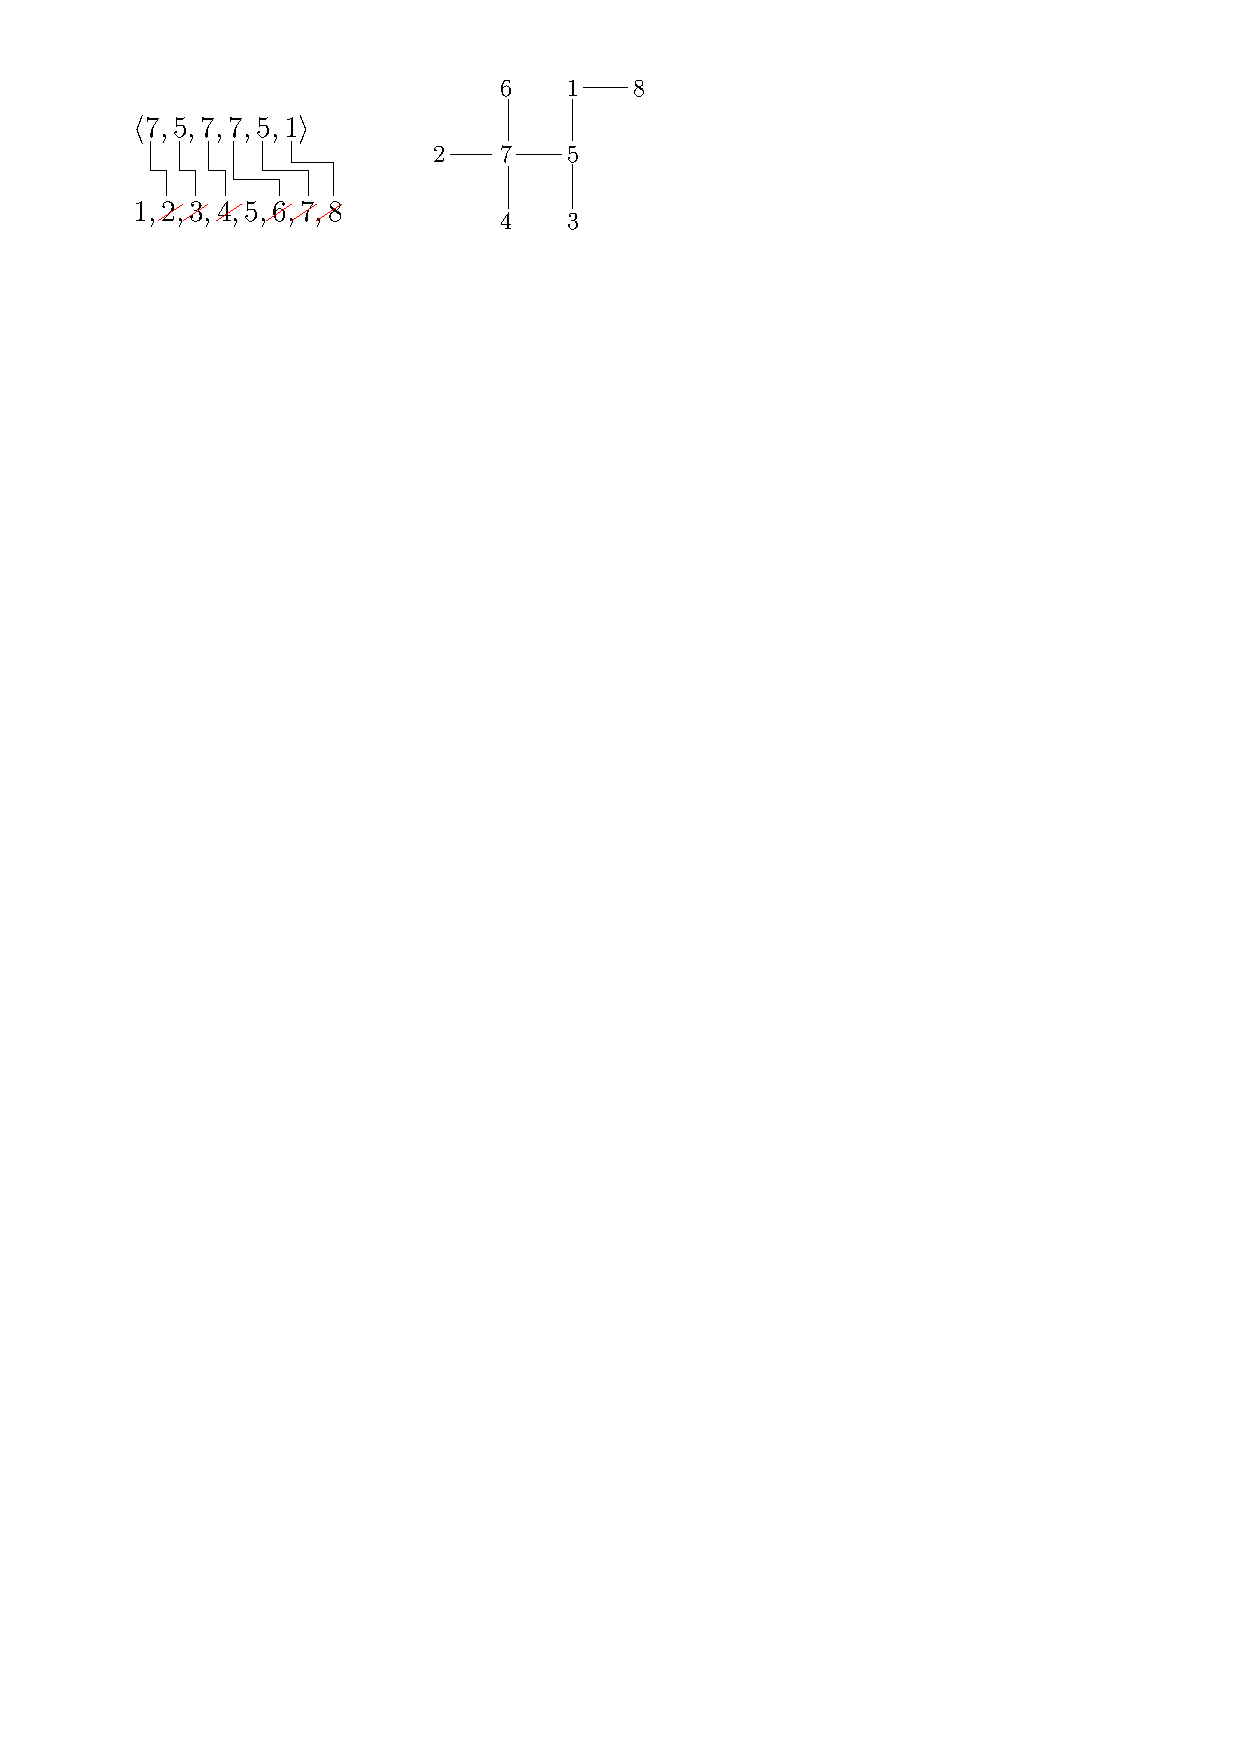
\includegraphics[width=0.5\linewidth]{figures/prufer-code-example.pdf}
    \caption{Example of a tree and its corresponding Prufer code}
    \label{fig:prufer-code-example}
\end{figure}

We can reverse the algorithm above to encode a tree into its Pr\"ufer code.

\begin{codebox}
    \Procname{$\proc{Prufer-Encode}(E)$}
    \li \For $i = 1$ \To $n-2$ \Do
        \li $s[i]$ = the unique vertex adjacent to the leaf with the smallest value
        \li remove the leaf with the smallest value
    \End
    \li \Return $s$
\end{codebox}

\subsection{Back to Counting Trees}

Each labeled tree with $n$ vertices has a unique Pr\"ufer's code of length $n-2$. Then, counting the number of labeled trees is equivalent to counting the number of Pr\"ufer codes for all the trees.

\begin{theorem}[Cayley's Formula]
    For each $n \geq 2$, there are exactly $n^{n-2}$ labeled trees on $\{1,\ldots,n\}$.
\end{theorem}

\begin{proof}
    To each tree, find the unique associated Pr\"ufer code $s:\; [n-2] \to [n]$. This creates a bijective correspondence between labeled trees and sequences $s:\; [n-2] \to [n]$.

    There are exactly $n^{n-2}$ such sequences and hence that many labeled trees on $\{1,\ldots,n\}$.
\end{proof}